\chapter{Introduction to GeomInt}

\section{Background} 

The use of the subsurface as a source of resources, a storage space and for installing underground municipal or traffic infrastructure has become much more intensive and diverse in recent years. In addition to classical anthropogenic interventions such as mining, oil and gas production or tunnel construction, other forms of underground use have come into the focus of economic, political and scientific research, particularly in connection with the transformation of energy systems. These include, for example, the extraction of energy (e.g. geothermal energy\index{geothermal energy}) and energy sources using new technologies (e.g. unconventional gas extraction\index{unconventional gas}) as well as the geological short-term and long-term storage of energy carriers (e.g. compressed air, hydrogen, methane) and the safe storage of waste generated during energy production or in other industrial sectors (e.g. carbon dioxide, radioactive waste\index{radioactive waste}).

Increasing utilization of the geological environment requires careful analyses of the rock-fluid systems as well as assessments of the feasibility, efficiency and environmental impacts of the technologies under consideration. The establishment of safe, economic and ecological operation of underground geosystems requires a comprehensive understanding of the physical, (geo)chemical and microbiological processes on all relevant time and length scales. This understanding can only be deepened on the basis of intensive laboratory and in-situ experiments in conjunction with reliable studies on the modelling and simulation (numerical experiments) of the corresponding multi-physical/chemical processes.

The rocks and rock mass themselves are characterized by complex material behaviour\index{complex material behaviour}. Irreversible deformation, rate-dependent strength behaviour as well as creep, swelling and shrinkage effects occur under real loading conditions. Damping aspects, for example in the range of low-frequency seismic waves, damage and physical-chemical aging (e.g. solution and/or precipitation reactions) play an important role in many geotechnical applications and have roots in the multiphase nature of geomaterials. In particular, the topics of damage, crack formation and propagation as well as interface problems are aspects that require further clarification. Because of prevailing knowledge gaps in these areas, many such processes can currently not be adequately modelled with commercial numerical simulation systems commonly used in geotechnical practice. They therefore represent topics in urgent need of research. The corresponding processes manifest themselves in diverse micro- and macromechanical behavioral structures of the considered materials and are here summarized under the umbrella term \textbf{discontinuities} (Fig.~\ref{fig:pro01}).

\begin{figure}[ht!]
\centering
%\includegraphics[width=1\textwidth]{figures/geomint-motivation}
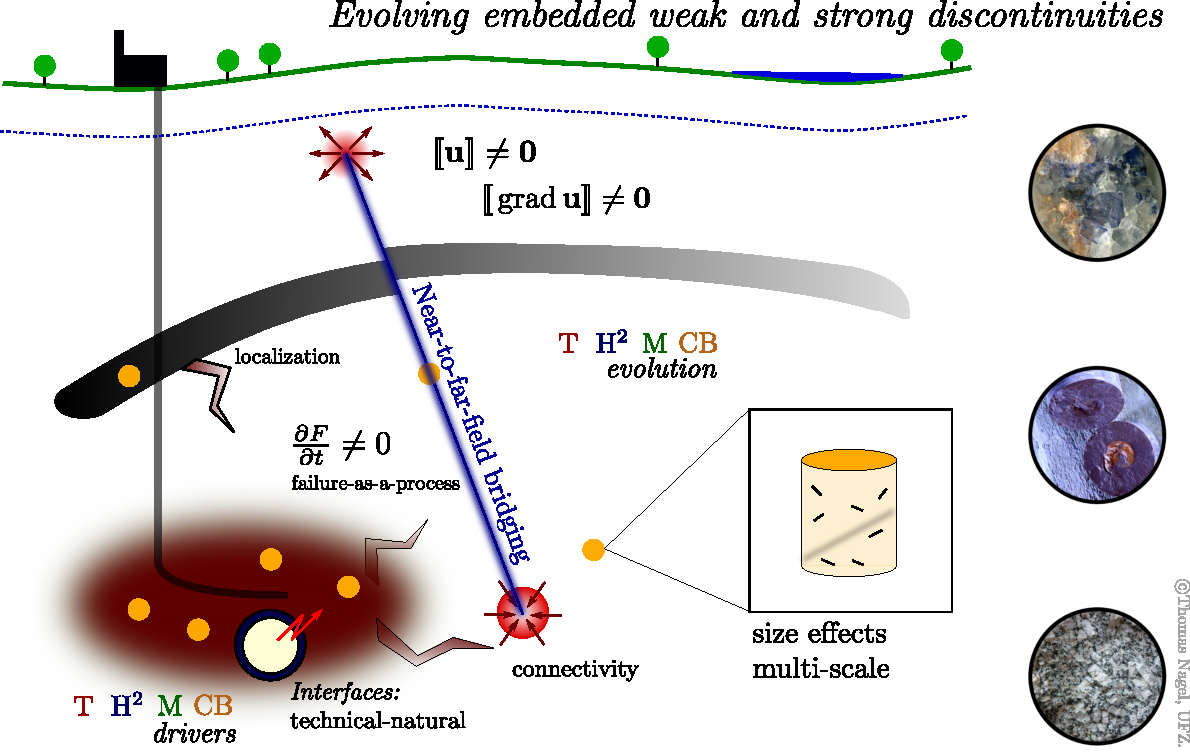
\includegraphics[width=1\textwidth]{figures/Barrier_concept.pdf}
\caption{Graphical abstract of the GeomInt project: geological reservoir-barrier systems and geomechanical integrity}
\label{fig:pro01}
\end{figure}

\section{The GeomInt project}
\label{sec:geomint}

GeomInt\index{GeomInt} (Geomechanical Integrity of Host and Barrier Rocks -- Experiment, Modeling and Analysis of Discontinuities) contributes to the realistic and application-oriented experimental-numerical analysis of the formation and development of discontinuities in underground rock salt\index{rock salt}, clay rocks\index{clay rock} and crystalline rocks\index{crystalline rock}. In the following, these rocks will also be briefly referenced as salt, clay and crystalline. The understanding and quantification of interactions with dynamically developing geological rock properties (e.g. permeability), which determine the geomechanical integrity\index{geomechanical integrity} and tightness of geological reservoir-barrier systems, are at the centre of this work. Included in the investigations are discontinuities of volumetrically distributed damage types as they occur in the damage zone of solid rocks, discontinuities that can form uncontrolled or controlled at phase boundary surfaces as well as discrete crack and fracture networks\index{fracture networks}. The pathways created or extended by these discontinuities for fluids in host and barrier rocks harbour the risk that, for example by migration of fluid phases from deep to near-surface geological strata and ultimately into the biosphere, vital ecosystems can be impaired significantly. A range of thermo-hydro-mechanical-chemical (THMC) processes\index{THMC processes} can cause an evolution of discontinuities in the near field of a geotechnical infrastructure. This in turn may lead to the establishment of previously not existent connectivity. When connectivity is established to conductive fault zones\index{fault zones} or fracture networks with a certain range, transport into the far field can become possible on a much shorter time scale than before (Fig.~\ref{fig:pro01}).

\begin{figure}[ht!]
\begin{minipage}{0.69\textwidth}
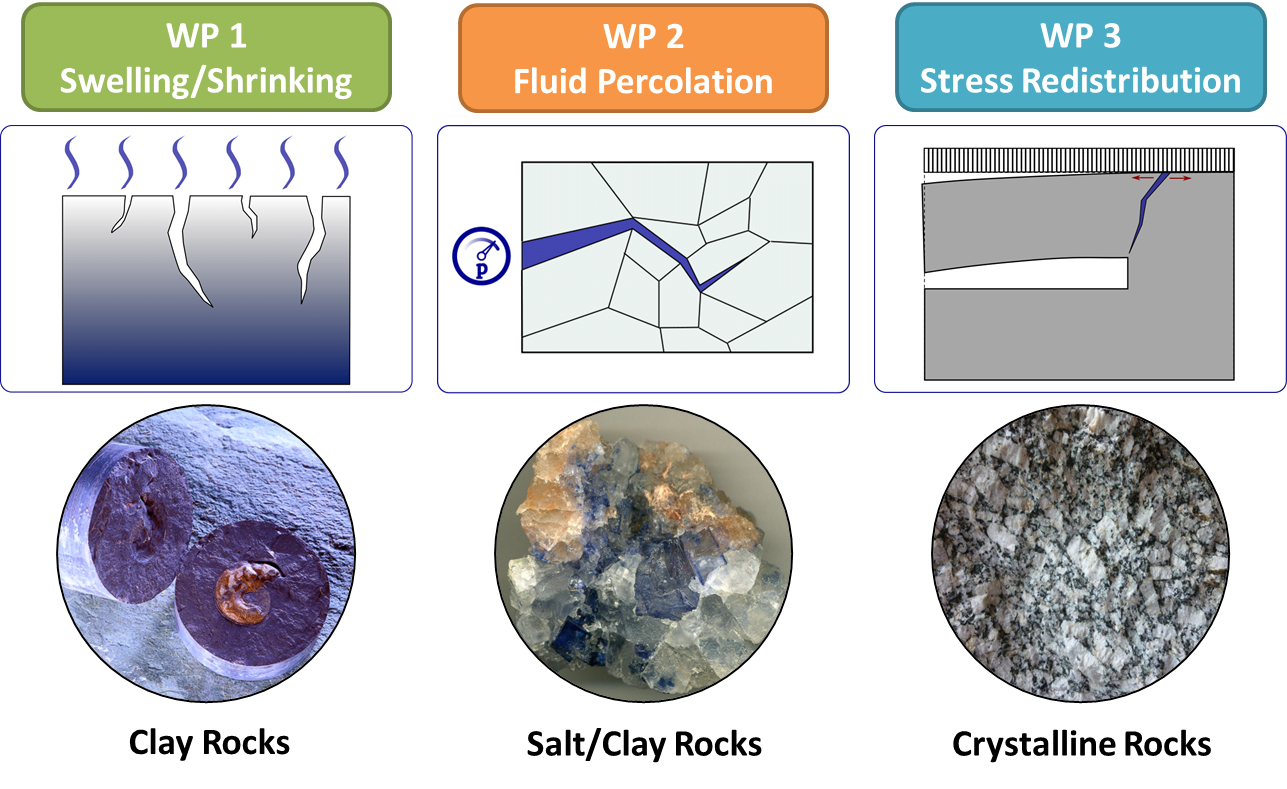
\includegraphics[width=1\textwidth]{figures/geomint-concept-02.png}
\end{minipage}
\hfill
\begin{minipage}{0.29\textwidth}
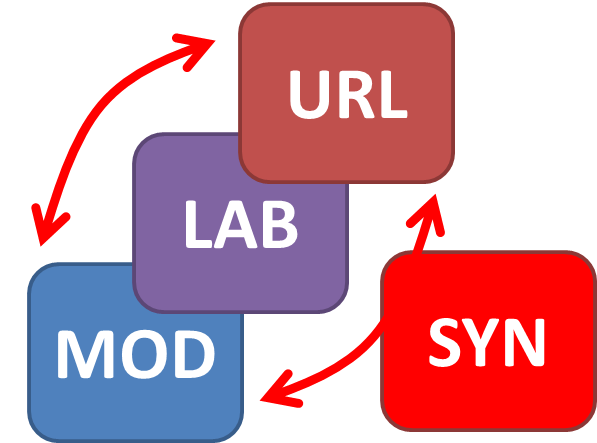
\includegraphics[width=1\textwidth]{figures/modal01a.png}
\end{minipage}
\caption{Work package structure of GeomInt according to process and rock types (left) and combining experimental as well as modelling works in a synergistic workflow (right)}
\label{fig:pro02}
\end{figure}

GeomInt is conducted by an interdisciplinary consortium of partners from universities, governmental and private research institutions with complementary, long-term experience in the analysis of underground geosystems. Three typical effects leading to the emergence and development of specific discontinuities are considered as main research areas: Swelling and shrinkage processes, pressure-driven fluid percolation and stress redistribution (Fig.~\ref{fig:pro02}). The research work is structured into laboratory experiments, numerical simulation and in-situ experiments (in underground research laboratories, URLs)\index{underground research laboratory}\index{URL}. New insights into process understanding have been gained from the laboratory experiments. In particular, contributions of coupled thermal, hydraulic, and mechanical (THM) processes for the formation and development of discontinuities have been considered. These findings have been used to support the further development of different continuum mechanical\index{continuum mechanics}, discontinuum mechanical\index{discontinuum mechanics} and hybrid numerical approaches\index{hybrid numerical approaches} and to compare their potentials and limitations. Novel models and algorithms have been implemented in scientific software mainly which is available to the research community. The suitability of the models for the analysis and prediction of realistic operating scenarios of underground geosystems (e.g. geothermal reservoirs, geological reservoirs for energy sources and waste) will be further validated on the basis of test field simulations of different in-situ experiments, which have been carried out primarily using synergies with other national and international research projects in underground laboratories accessible to project partners of GeomInt.
%
The process-oriented work packages are interlinked with synthesis activities such data and model integration using virtual reality (VR) methods (Fig.~\ref{fig:pro03})\index{Virtual Reality (VR)}. A corresponding pilot demonstrator is being implemented in the Mont Terri project.

\begin{figure}[ht!]
\begin{minipage}{0.49\textwidth}
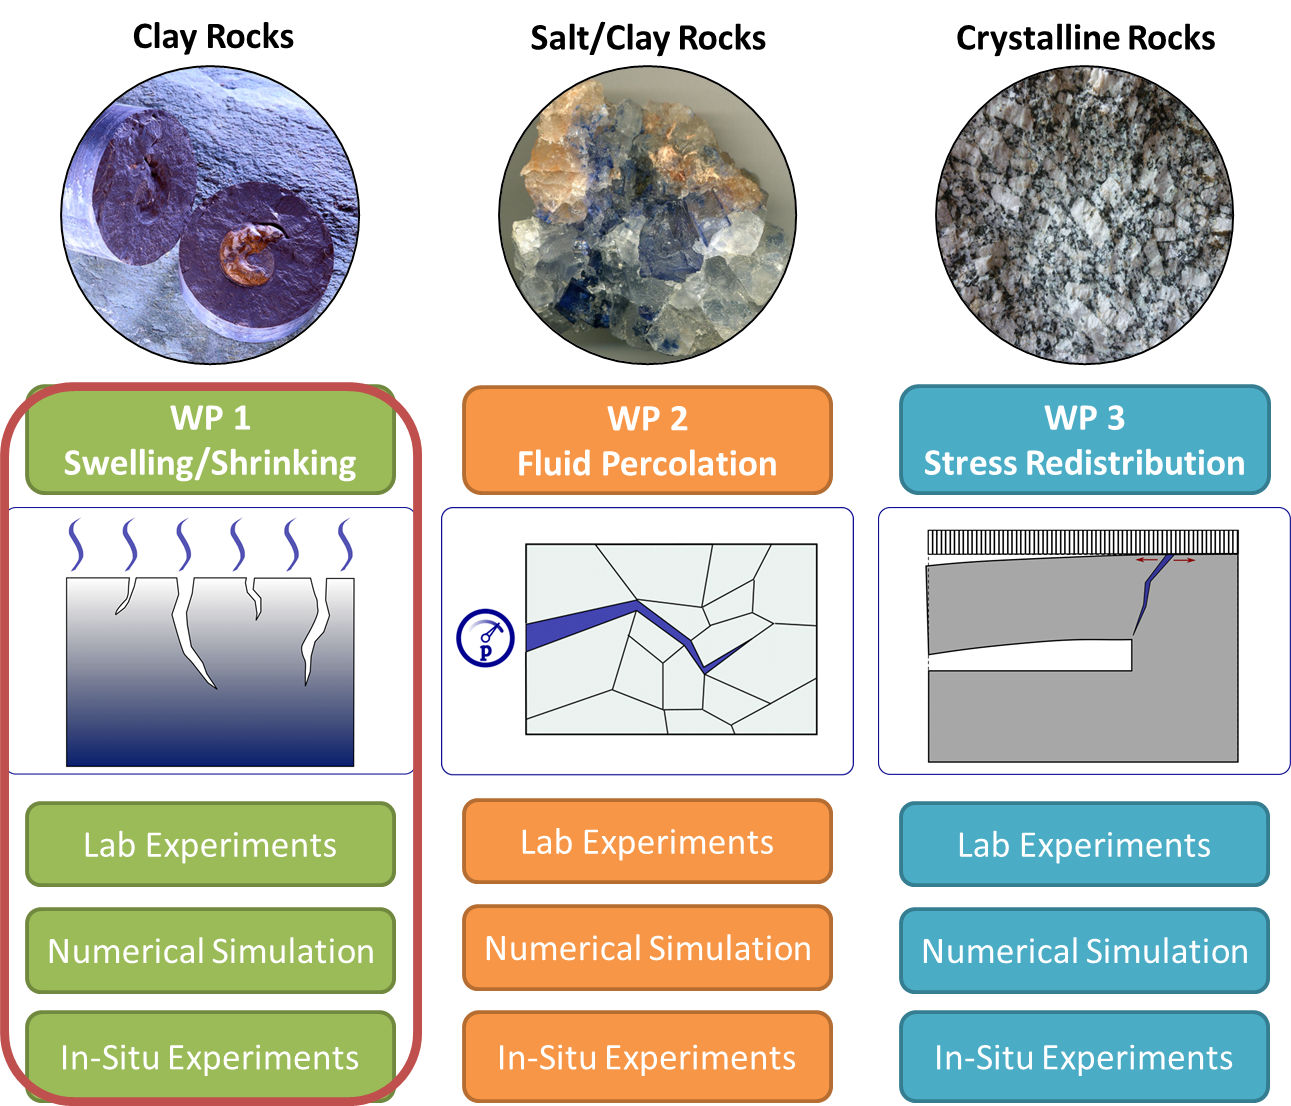
\includegraphics[width=1\textwidth]{figures/geomint-wp1a.png}
\end{minipage}
\hfill
\begin{minipage}{0.49\textwidth}
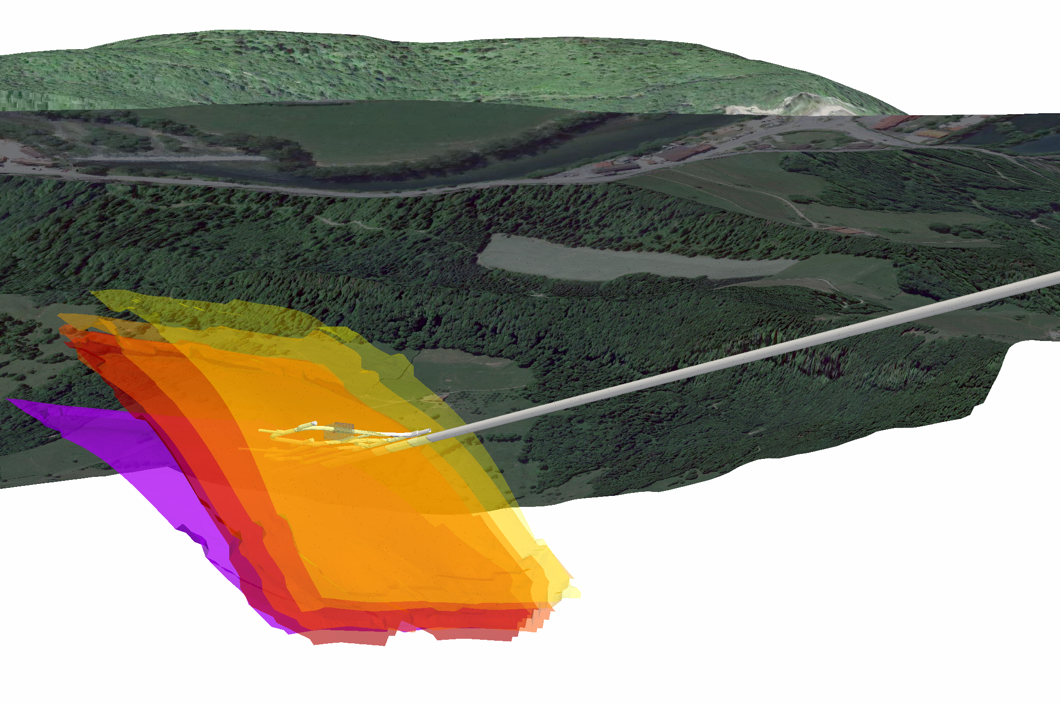
\includegraphics[width=1\textwidth]{figures/mt-vr-01.png}
\end{minipage}
\caption{Synthesis: Interlinking process-oriented work packages with VR methods (VR Mt. Terri - visual data and model integration)}
\label{fig:pro03}
\end{figure}

The project results allow an improved process understanding. The applied methods and the application-oriented systems for relevant time and length scales will support safer, more reliable and more efficient planning and realization of geotechnical applications. An important advantage of GeomInt is the principle transferability of experimental-numerical concepts, models and methods to a multitude of urgent scientific-technical questions in the geosciences. This allows the exploitation of project results for different politically and socially relevant geotechnological uses (e.g. deep geothermal energy, energy storage, repository problems, methods for hydraulic stimulation, conventional and unconventional resource extraction or tunnel construction). This transferability has been particularly taken into account in the methodological design of the project as well as in the documentation of methods, approaches and results and can at the same time serve as a basis for potential follow-up work to GeomInt.\index{Virtual URL Mt. Terri}

\section{GeomInt approach: lab, in-situ, in-silico, virtual reality}\index{in-situ}\index{in-silico}

GeomInt relies on a very close link between experimental and modelling work. Three work packages focus on different mechanisms affecting the barrier integrity of potential host rocks: (WP1) swelling/shrinking of clays, (WP2) pressure driven fluid percolation in salt and clay rocks as well as (WP3) stress redistribution in crystalline rocks.
%
Fig.~\ref{fig:appraoch} illustrates the geographical WP workflows from in-situ sampling to geomechanical laboratories and modelling. The main sources for rock samples are (i) Mt. Terri for clay (ii) Springen for salt and (iii) Freiberg/Kirchberg for crystalline rock specimen. Moreover, there is collaboration with other URLs (Bure, Grimsel) concerning experimental and modelling work -- mainly for testing transferability of the methodology to other rock types (e.g. Callovo-Oxfordian Clay - COx).\index{URL Mt. Terri}\index{URL Reiche Zeche}\index{URL Bure}\index{URL Grimsel}\index{Callovo-Oxfordian Clay (COx)}

\begin{figure}[ht!]
\centering
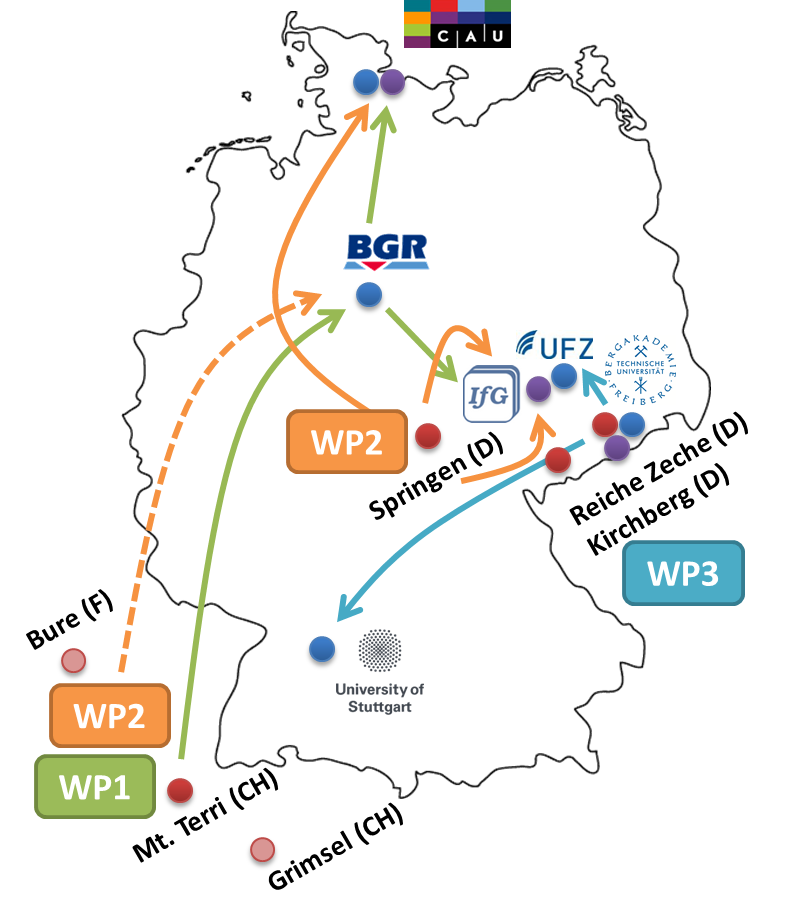
\includegraphics[width=0.8\textwidth]{figures/geomint-all.png}
\caption{Geographical work flow including interlinked experimental and modeling works in GeomInt}
\label{fig:appraoch}
\end{figure}

In the following we briefly introduce the ''geographical workflow'' for the individual work packages. Please not that the experimental and modelling platforms for the analysis of discontinuities are being established independent of specific rock types.

\begin{figure}[ht!]
\begin{minipage}{0.48\textwidth}
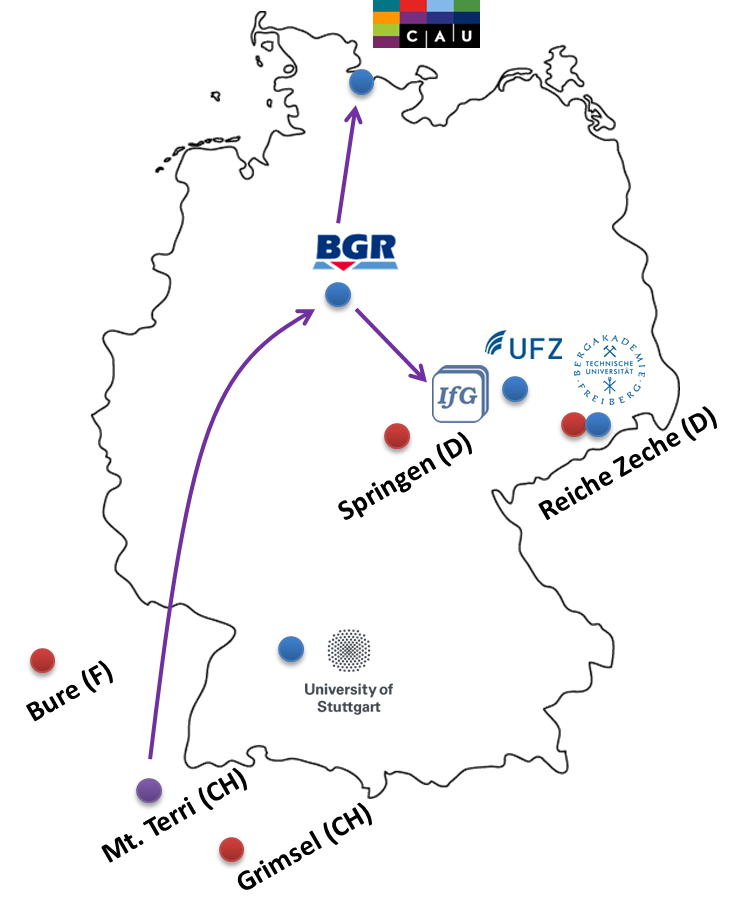
\includegraphics[width=\textwidth]{figures/geomint-wp1.png}
\caption{WP1: Swelling / shrinking}
\end{minipage}
\hfill
\begin{minipage}{0.48\textwidth}
WP1 is dealing with swelling and shrinking processes in clay stone. BGR obtains \textbf{Opalinus clay} samples from the Mont Terri Underground Research Lab (URL) in Switzerland and providing them for laboratory testing to CAU and IfG partners in Kiel and Leipzig, respectively. Samples come from various clay and sandy facies. Experimental work with specimen from the sandy facies is particularly challenging due to the large heterogeneity of the material. WP1 is closely linked with the Mont Terri Project in cooperation with swisstopo.\index{Opalinus clay}
\end{minipage}
\end{figure}

\begin{figure}[ht!]
\begin{minipage}{0.48\textwidth}
Fluid percolation processes are studied in both \textbf{clay and salt rocks}, i.e. ductile materials. Samples of Opalinus clay come from the Mt. Terri URL (see above). Salt rock samples are mainly obtained from the Springen site in Thuringia. Experimental works concerning percolation are conducted in the IfG and CAU labs in Leipzig and Kiel. WP2 investigates mechanisms of percolation threshold for both rock types depending on hydro-mechanical (HM) processes (i.e. fluid pressure and mechanical stress field).
\end{minipage}
\hfill
\begin{minipage}{0.48\textwidth}
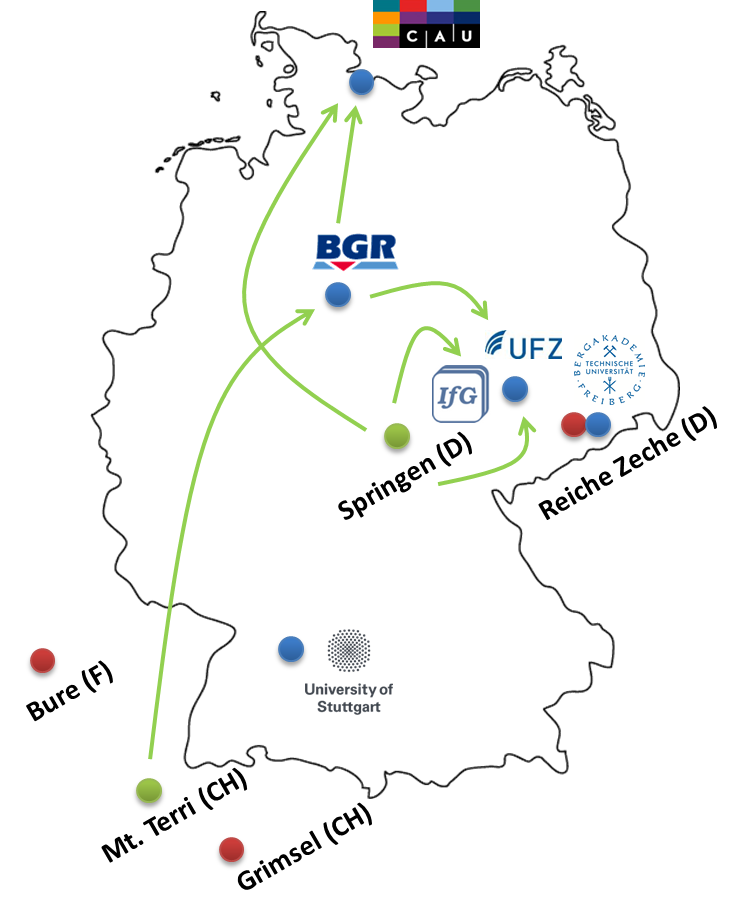
\includegraphics[width=\textwidth]{figures/geomint-wp2.png}
\caption{WP2: Fluid percolation}
\end{minipage}
\end{figure}

\begin{figure}[ht!]
\begin{minipage}{0.48\textwidth}
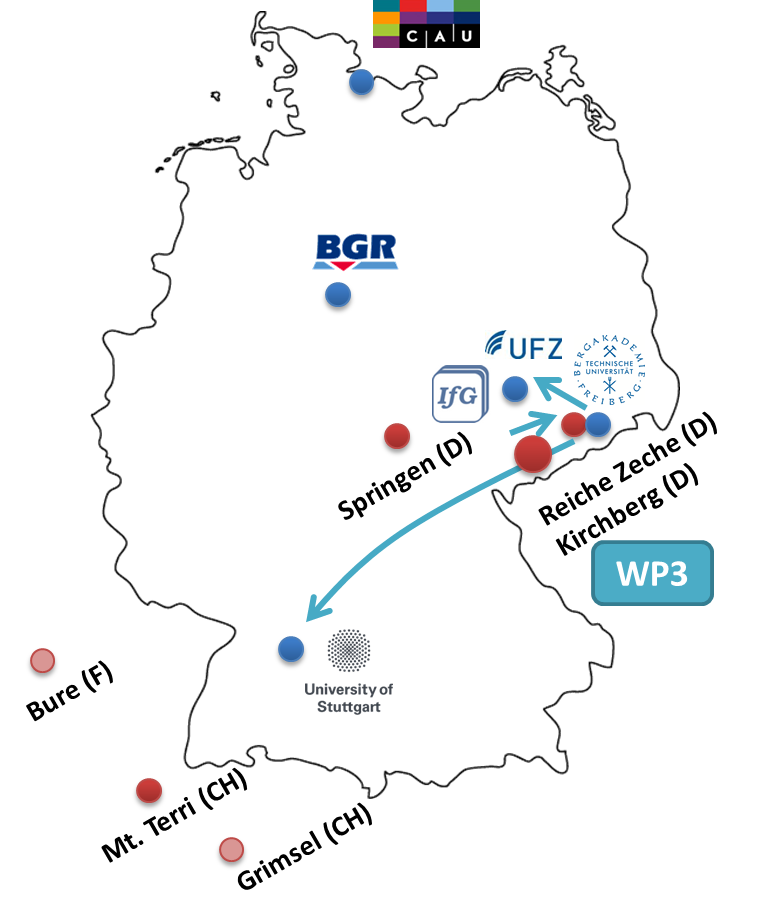
\includegraphics[width=\textwidth]{figures/geomint-wp3.png}
\caption{WP3: Stress redistribution}
\end{minipage}
\hfill
\begin{minipage}{0.48\textwidth}
WP3 is investigating discontinuities formed by stress redistribution in brittle materials. \textbf{Granite rock} samples are obtained from locations in the Ore Mountains, i.e. from Kirchberg and Freiberg (URL Reiche Zeche). Experimental  investigations are conducted in the Freiberg (TU Freiberg) and Stuttgart labs (University of Stuttgart). Constant Normal Load (CNL) and Constant Normal Stiffness (CNS) experiments are conducted to study fluid flow in rough fractures under confining stresses. Rock samples from Freiberg will be also used with in the ''Crystalline Task'' of the new DECOVALEX-2023 phase.\index{Constant Normal Load (CNL) experiment}\index{Constant Normal Stiffness (CNS) experiment}\index{DECOVALEX}
\end{minipage}
\end{figure}

Output from the following research infrastructures will be combined:
\begin{itemize}
    \item \textbf{Rock-mechanical laboratories}
	\begin{itemize}
		\item THM-coupled testing under controlled boundary conditions
		\item Material and process characterization
	\end{itemize}
	\item \textbf{Numerical methods and software}
	\begin{itemize}
		\item OpenGeoSys (XFEM, PFM)
		\item md-LEM (LEM)
		\item pythonSPH (SPH)
		\item UDEC, 3DEC (DEM)
		\item FLAC3D (FDM)
	\end{itemize}
	\item \textbf{Underground laboratories}
	\begin{itemize}
		\item Springen (rock salt, potash)
		\item Mont Terri (clay rock)
		\item Reiche Zeche (crystalline rock)
	\end{itemize}
	\item \textbf{Simulation- and development infrastructure}
	\begin{itemize}
		\item HPC Cluster
		\item Version management
		\item VISLAB (\url{www.ufz.de/vislab})
	\end{itemize}
\end{itemize}

In addition to experimental (lab and in-situ) and modelling work, we use Virtual Reality (VR) methods for data and model integration as well as visualization. Fig. \ref{fig:vr-url} shows a snapshot of the Virtual URL project for Mont Terri. The basic idea is to combine all information from in-situ (and even lab) experiments as well as the corresponding models in a Virtual Reality context - like a visual data base. VR embedded data can be accessed in an interactive and interoperable manner \cite{Rink2020}.
\index{High-Performance-Computing (HPC)}\index{VISLAB}

\begin{figure}[ht!]
\centering
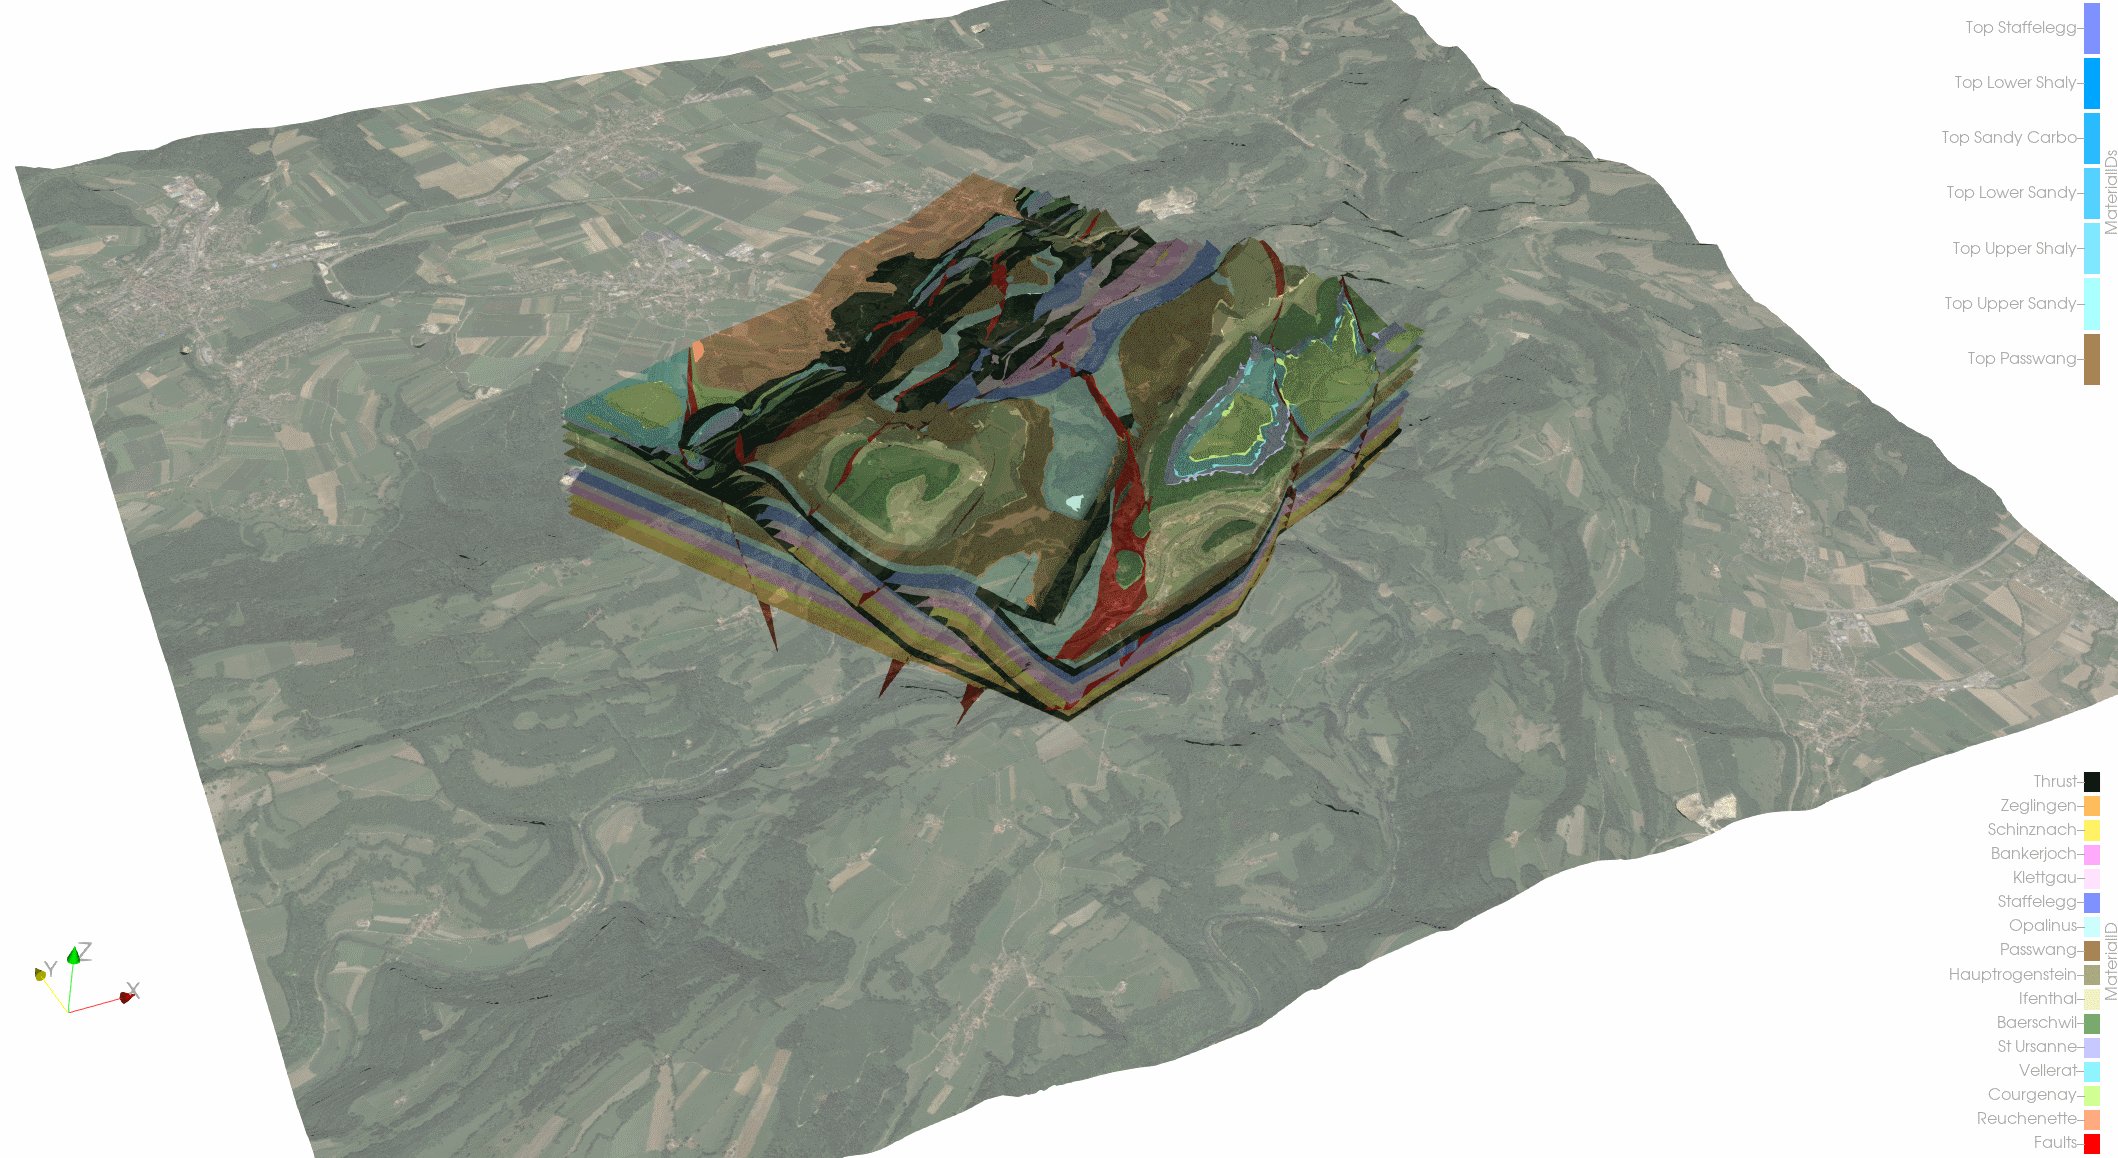
\includegraphics[width=0.9\textwidth]{figures/mt-surface+move.png}
\caption{Virtual URL Mont Terri: Virtual data and model integration in a precise geo-referenced context}
\label{fig:vr-url}
\end{figure}

Experimental and modelling platforms are described in detail in Chapter \ref{cha:exp} and \ref{cha:num}, respectively.

\clearpage
%--------------------------------------------------------------------
\section{GeomInt team}
\label{sec:team}

The GeomInt consortium is made up of the partners Federal Institute for Geosciences and Natural Resources, Christian-Albrechts-University of Kiel, Helmholtz Centre for Environmental Research - UFZ, Institut f\"ur Gebirgs\-mechanik GmbH, TU Bergakademie Freiberg and University of Stuttgart. The consortium is based on the complementary expertise and resources of the partners, partly unique laboratory equipment, many years of experience with different numerical approaches and access to underground laboratories for the rocks under consideration. Detailed information on the partners and their previous project-relevant work is presented in the following.

\subsection{BGR}
\begin{wrapfigure}{r}{2cm}
\centering
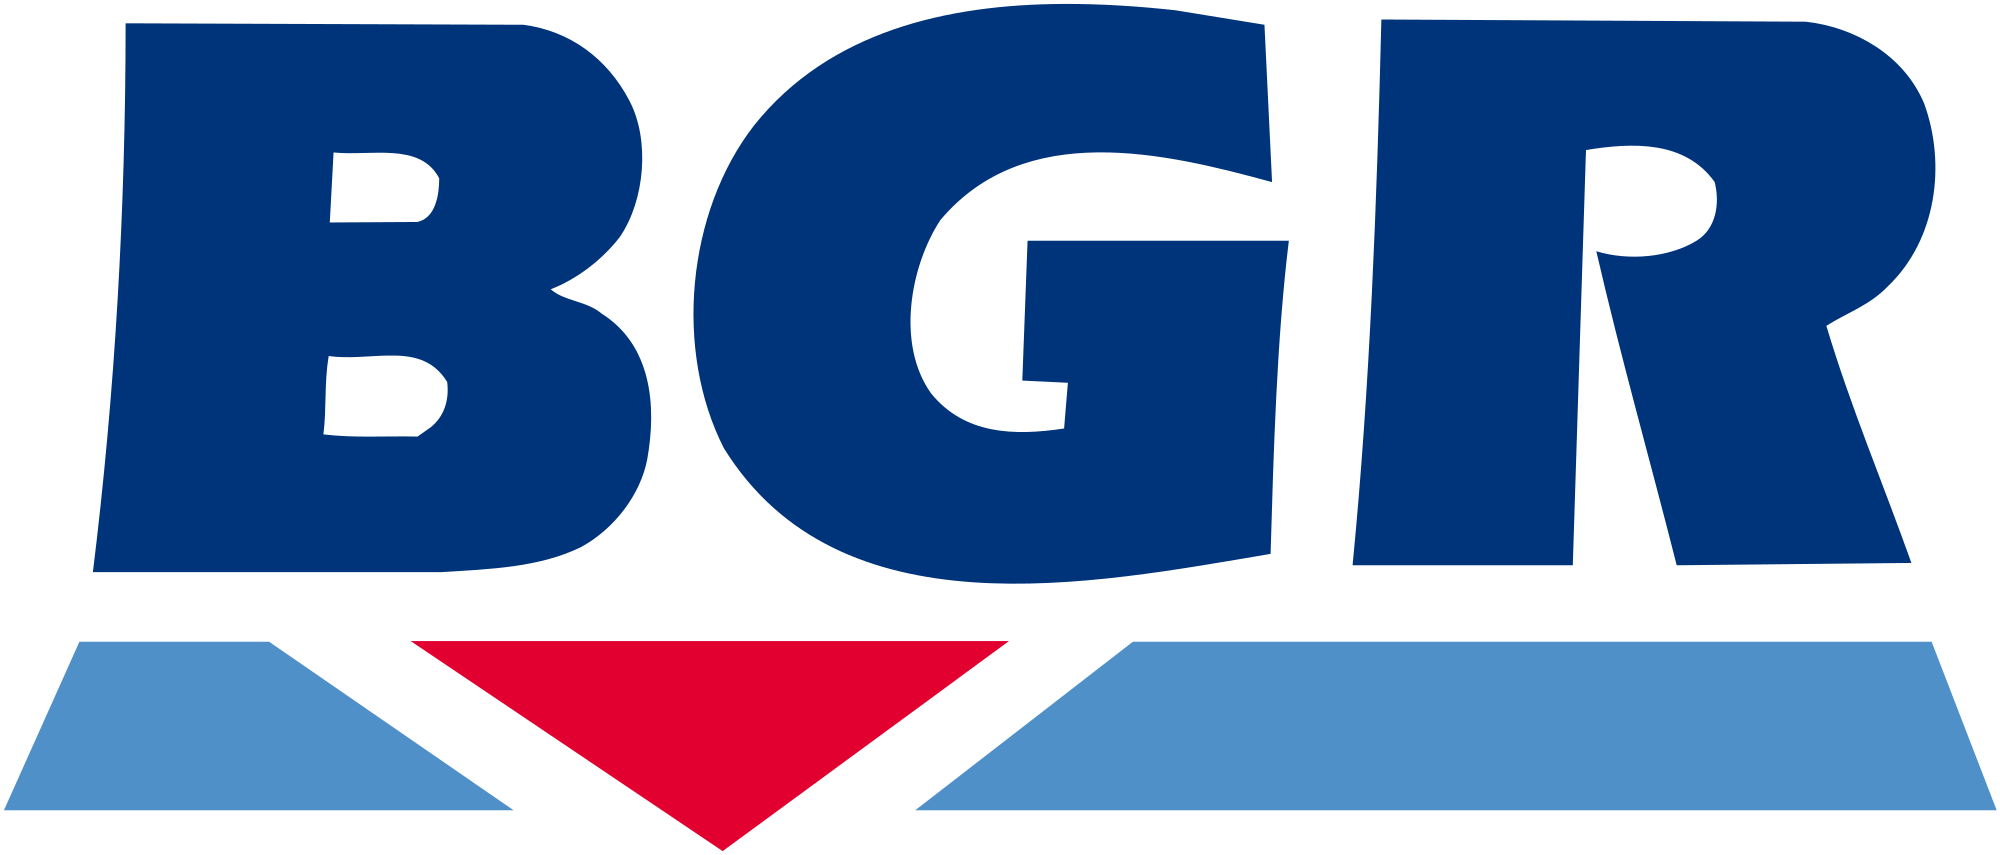
\includegraphics[width=2cm]{./figures/BGR_Logo.png}
\end{wrapfigure}
The Federal Institute for Geosciences and Natural Resources (BGR, Germany) is the central consulting institution for the German federal government for all geoscientific questions, inter alia the safe final disposal of radioactive waste and the related geological-geotechnical safety analyses. As such, the BGR with its wide-ranging experience has an interest in investigating the host rocks salt, claystone and crystalline rocks to guarantee an independent recommendation for the site selection process. This includes the use of state-of-the-art modelling and experimental techniques. Within the GeomInt project, the BGR is focusing on the integrity of clay rock formations as they are currently investigated in the Mont Terri Underground Rock Laboratory (URL) in Switzerland. The BGR is currently coordinating and participating in several experimental campaigns that are expected to enhance the fundamental understanding of clay rock exposed to stress redistribution, seasonally varying boundary conditions and pressure driven percolation. For the simulation of the hydraulic conditions of unsaturated claystone coupled with unsaturated linear elastic mechanical deformation, a strong collaboration with the Helmholtz Centre for Environmental Research (UFZ) has been pursued to employ the open source code OpenGeoSys for in-situ scale problems of the Mont Terri URL.

\subsection{CAU}
\begin{wrapfigure}{r}{2cm}
\centering

\includegraphics[width=2cm]{./figures/cau_logo.png}
\end{wrapfigure}

The geomechanical and geotechnical group of Christian-Albrechts-University (CAU) of Kiel has vast experience in the experimental and numerical analysis of coupled thermo-hydro-mechanical (THM) processes in geomaterials. Some research fields which are under investigation and development at CAU Kiel are: material characterization by static, cyclic and dynamic loaded soil-structure-interaction, development of sustainable geomaterial and earth structure, material characterization by geophysical and advanced geotechnical methods, energy geotechnics, energy geo-storages, and cyclic thermo-hydro-mechanical loaded geomaterial. In 2016, the first international conference on energy geotechnics (ICEGT-2016) was organized and hosted in Kiel University. The numerical simulations such as Coupled hybrid models, boundary element modeling (BEM), finite element modeling (FEM), static and dynamic soil-structure-interface and constitutive modeling, cyclic system / macro modeling for complex soil-structure-conditions and loads as well as fracture simulation under coupled THM processes using lattice element method (LEM) have all been developed here and have been applied in different research fields and projects, such as ANGUS, DuoFill, FIBERSLAG, BioSolidEncap and GeomInt.

\subsection{IfG}
\begin{wrapfigure}{r}{2cm}
\centering

\includegraphics[width=2cm]{figures/logo-ifg-klein.png}
\end{wrapfigure}
The Institut f\"ur Gebirgsmechanik GmbH - IfG is one of the leading companies for all questions regarding the use of salt formations, e.g. salt mining, storage, and waste disposal projects. We adopt an interdisciplinary approach, consisting of numerical and experimental geomechanics, as well as geotechnical in in-situ field measurements. The company provides fundamental geomechanical/geotechnical safety concepts, and produces evidence reports on rock-mechanical stability and long-term safety in the form of design concepts, site planning procedures and public acceptance procedures. Supported by combinations of in situ observations, 
geomechanical laboratory testing and numerical modelling we provide comprehensive expertise in rock mechanics, necessary to solve practical mining or repository problems and to reduce project risks. Our research includes such diverse phenomena like creep, strain softening and post-failure behavior, rock burst mechanisms, and pressure-driven percolation in polycrystalline salt rocks (both numerically and experimentally). Overall, the IfG can draw on more than five decades of continuous application of research in the field of rock mechanics.

\subsection{TUBAF}
\begin{wrapfigure}{r}{2cm}
\centering
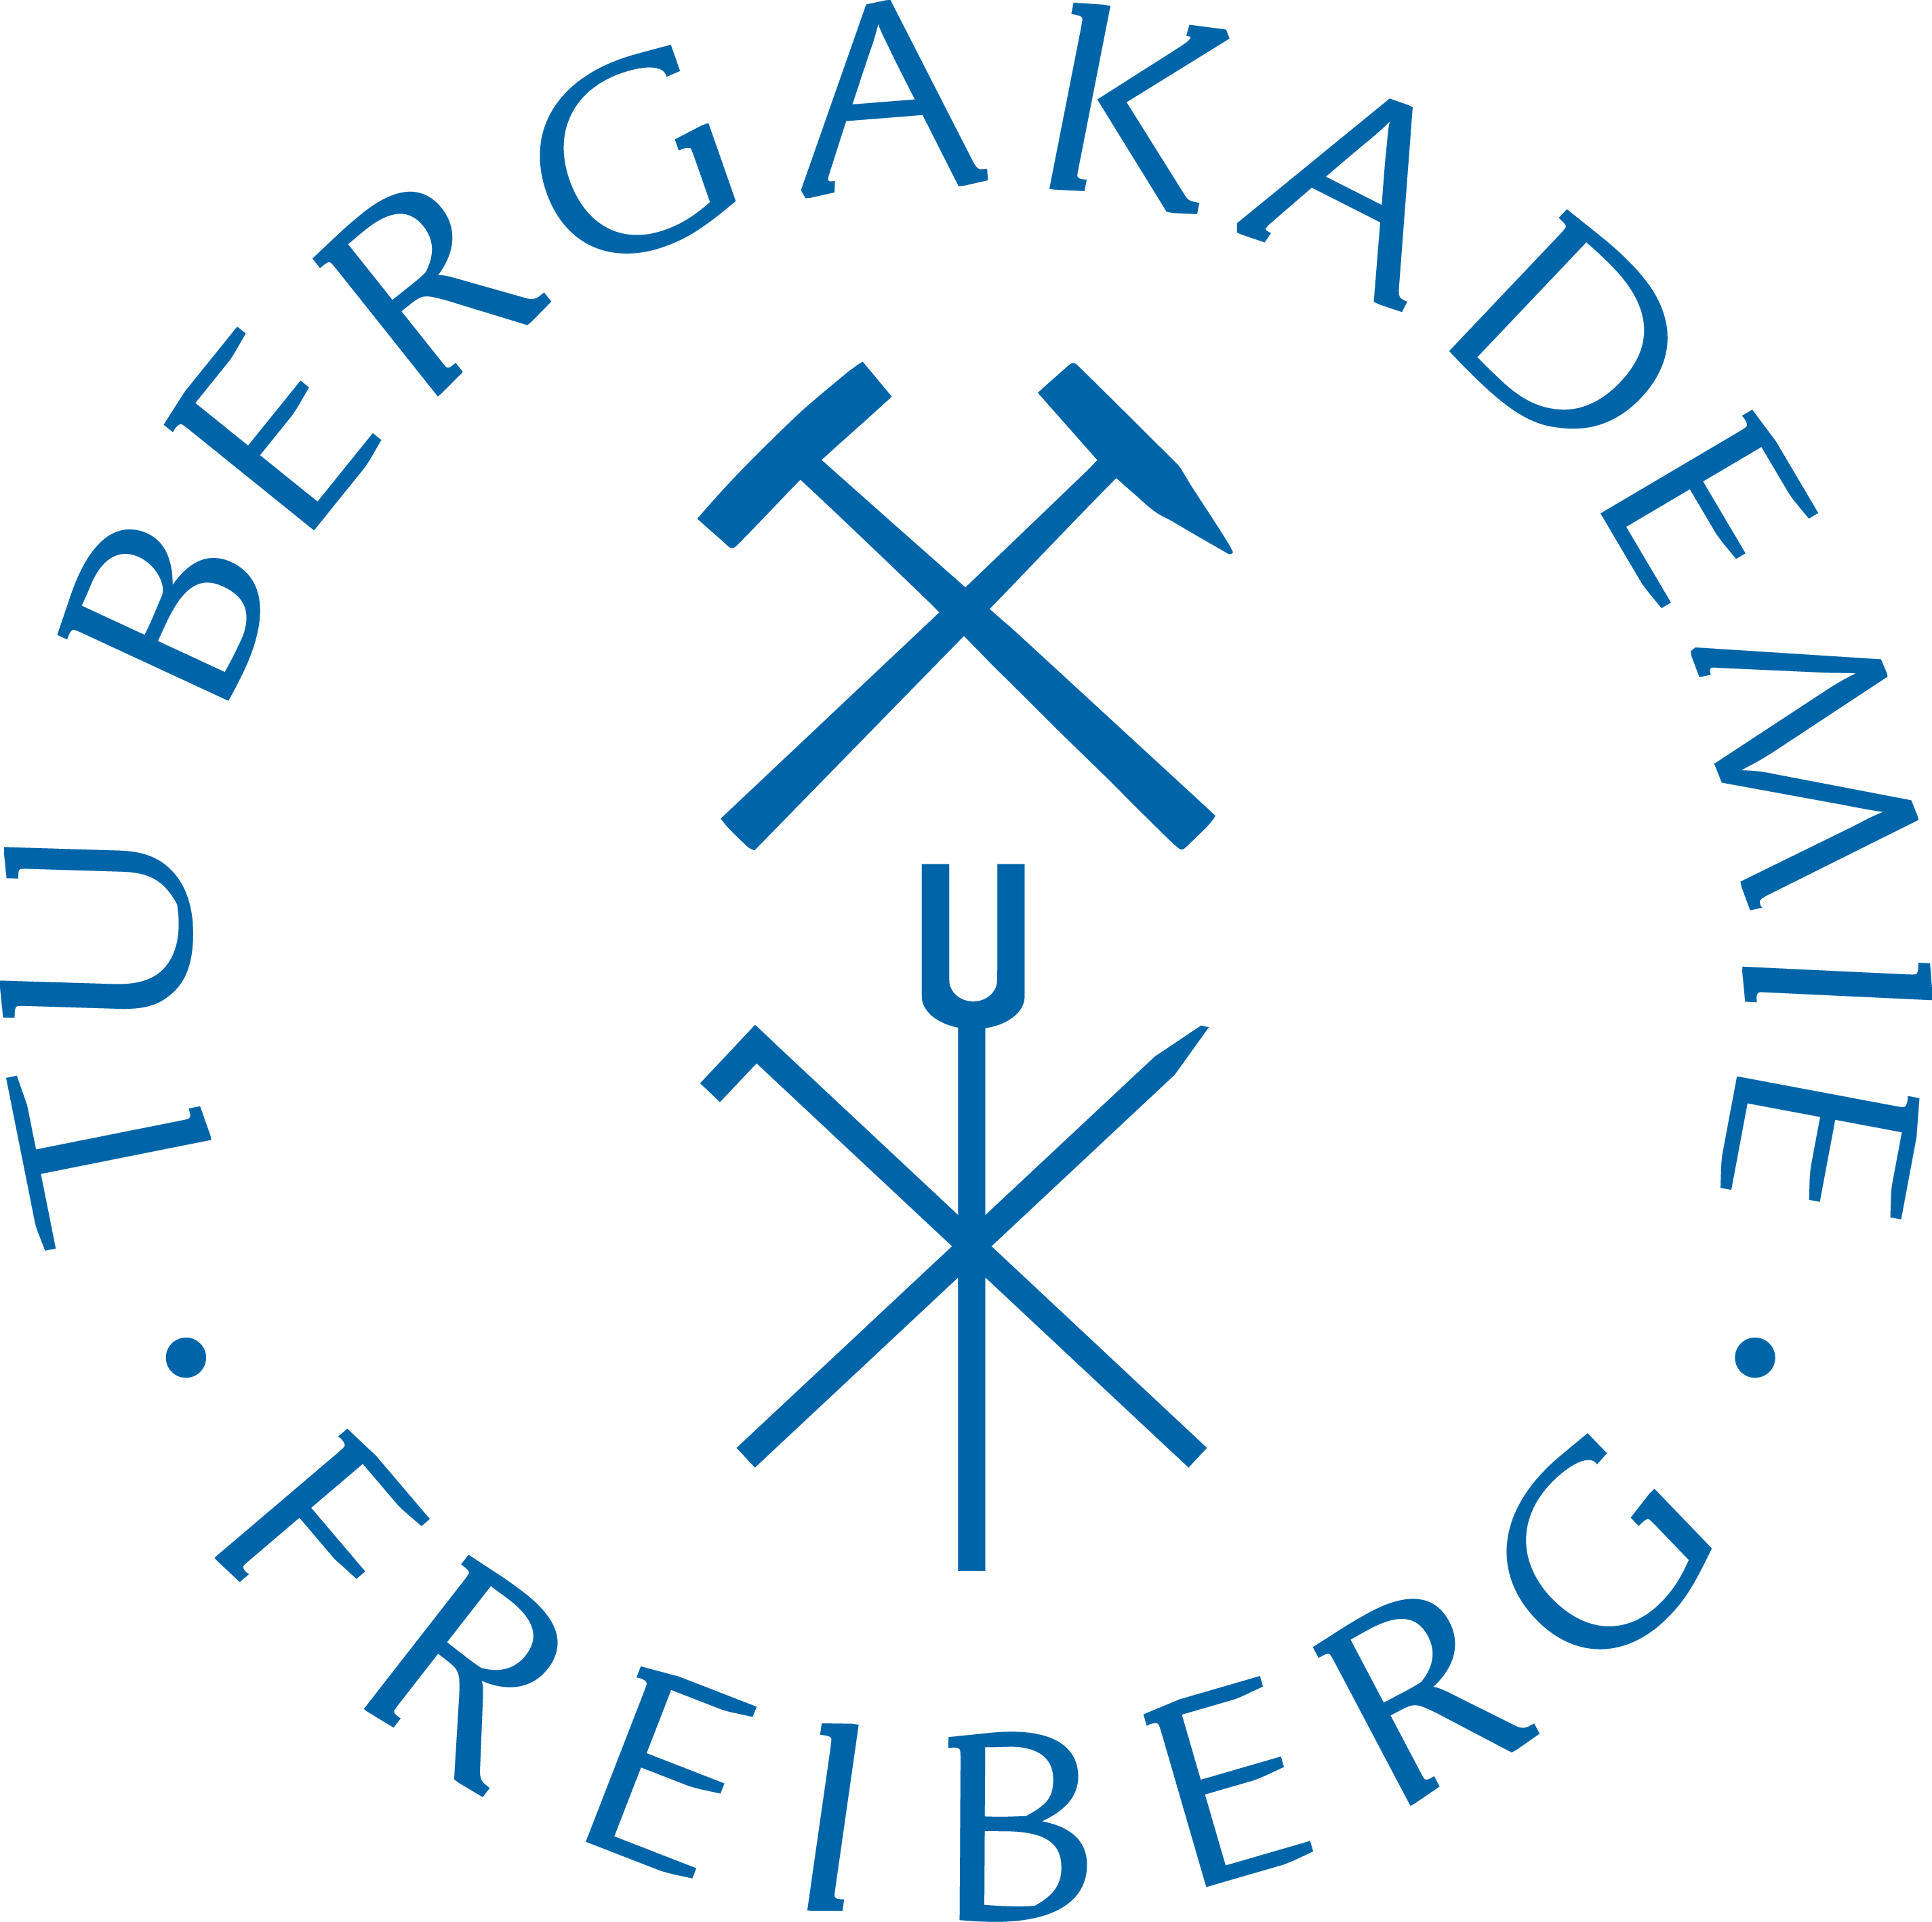
\includegraphics[width=2cm]{figures/TUBAF_Logo_orig_RGB}
\end{wrapfigure}
The Technical University of Freiberg as so called "University of Resources" focuses on energy, resources and materials. The institute of geotechnical engineering works in the field of using the crust of the earth. This affects topics like radioactive waste repositories in different host rocks (salt, crystalline, clay), geothermal energy production, gas storage or tunneling. To face this challenges the results of the rock mechanical laboratory, the "Reiche Zeche" (the local research mine) and numerical simulations are used. Involving practical and numerical results on different scales helps to give a useful contribution to open questions in the related research topics. The staff of the institute works in different national and international research projects. The topic of deep geothermal energy is on the agenda since 2008. Particularly the genesis and development of cracks and crack formations was intensively studied. E.g. the hydraulic fracturing, the induced seismicity or the response of existing cracks to static and dynamic loads have been experimentally and numerically investigated.  

\subsection{UFZ}
\begin{wrapfigure}{r}{2cm}
\centering
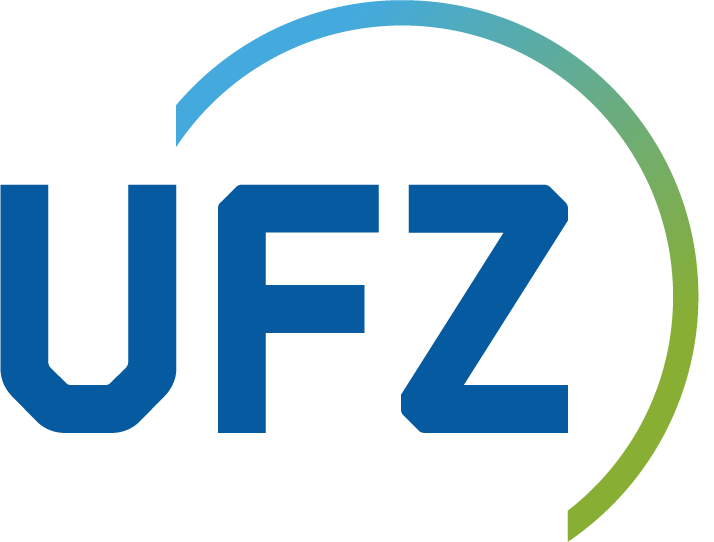
\includegraphics[width=2cm]{figures/ufz}
\end{wrapfigure}
The Helmholtz Centre for Environmental Research - UFZ deals with a variety of tasks in environmental, climate and energy research, the results of which are internationally recognized. In the energy sector, the spectrum of topics covered ranges from process modelling and simulation to the development of innovative monitoring strategies and the investigation of socio-economic aspects. Since its foundation in 2007, the Department of Environmental Informatics (ENVINF) has been concerned with the development of numerical methods and software components for the simulation of coupled processes in porous media based on the finite element method. In addition, the development of simulation platforms for the treatment of these problems as well as benchmarking for model and software validation will be discussed. Workflows and system components for the 3D visualization of complex, heterogeneous data from different sources are an integral part of these platforms. In this context, the UFZ acts as main developer and coordinator of the international scientific open source software project OpenGeoSys. In addition to method and software development, there is a strong connection to applications in hydrology, geotechnics and energy storage research. Aspects of modelling and numerical simulation of discontinuities in rocks were considered in phase field, non-local deformation and modified XFEM approaches, especially in connection with process analysis in Enhanced Geothermal Systems. In order to increase the efficiency of numerical simulations and for the clear evaluation of results, the UFZ has capacities for high-performance computing and scientific 3D visualization. 

\subsection{UoS}
\begin{wrapfigure}{r}{2cm}
\centering

\includegraphics[width=2cm]{figures/unistuttgart_logo.png}
\end{wrapfigure}
The Institute of Applied Mechanics (Chair of Continuum Mechanics) at the University of Stuttgart (UoS) contributes with a profound knowledge of coupled geomechanical problems in different scales. Investigations in the field of subsurface flow in fractured and unfractured porous media to answer open questions regarding underground storage, geomaterial characterization and geotechnical energy and safety concerns is just a small selection of the overall research fields of interest. Experimental state of the art infrastructure including a custom designed $\mu$XRCT-Scanner with for image-based characterization combined with hydro-mechanical in-situ experiments, imaging and PIV of complex single and multi-phase flow processes in micro-fluidic setups with sub-micrometer pore-scale resolution and various experimental devices for the harmonic characterization of complex fluids, solids, and especially rock (and granular media) samples form the basis of the so called Porous Media Lab(oratory) at UoS. The tight interplay of experimental and theoretical work is closed by a number of advanced numerical in house codes such as the solver package HOOSPH (based on the HOOMD-blue library), a massive parallel CPU/GPU Smoothed Particle Hydrodynamics (SPH) framework, PANDAS a general Finite Element (FE) package for strongly coupled multiphasic porous media problems, and a newly developed extension of the DUNE PDELab framework for coupled problems in fractured porous media using hybrid-dimensional element formulations. Important contribution of the experimental and numerical work in numerous projects within the CRC 1313 at University of Stuttgart (https://www.sfb1313.uni-stuttgart.de), GeomInt (https://www.ufz.de/geomint/), SHynergie and the Cluster of Excellence SimTech (https://www.simtech.uni-stuttgart.de) help to prove the deep understanding of geomechanical processes.